\section{Binary--mixture periodic in 3-dimensions}
The existence of a temperature gradient in the system should not be able to generate a net flow in the fluid. 
This point is discussed by Levich who describes how the flow at the interface should be accompanied by a back-flow in the bulk fluid.\cite{Levich}
In the case of the binary--mixture held between two walls, the walls are held stationary and provide a momentum sink which allows a net flow to exist within the fluid.
To replicate the behaviour described by Levich one must study a system with no such momentum sinks, for example a simple periodic system of two immiscible fluids as shown on the left--hand side of Figure \ref{SetUp}.

This system was prepared from a FCC lattice of Lennard--Jones particles and the parameters described in Section \ref{InteractionModel} and using a Nos\'e--Hoover thermostat and barostat.
To create the fluid state, the systems were equilibrated for $2 \times 10^{6}$ timesteps (of length $\delta t = 0.001\ \tau$) at a pressure of $P^{*} = 0.1$ and temperatures of $T^{*}=0.8$ and $T^{*}=0.9$.

\subsection{Comparing the Virial and Irving--Kirkwood stress}
Once again there is an ambiguity over which stress--tensor should be used for calculating the fluid stress profile.
Initially, both $\sigma^{\mathrm{V}}$ and $\sigma^{\mathrm{IK}}$ were computed for the symmetric--binary mixture.
This was achieved by running the equilibrated systems for $10 \times 10^{6}$ timesteps over which period the number--density, $\sigma^{\mathrm{V}}$ and $\sigma^{\mathrm{IK}}$ were calculated for 400 spatial bins.
As discussed before, the Irving--Kirkwood analysis was very computationally expensive and this simulation length was the upper feasible limit.
\FloatBarrier

\begin{figure}[h]
\centering
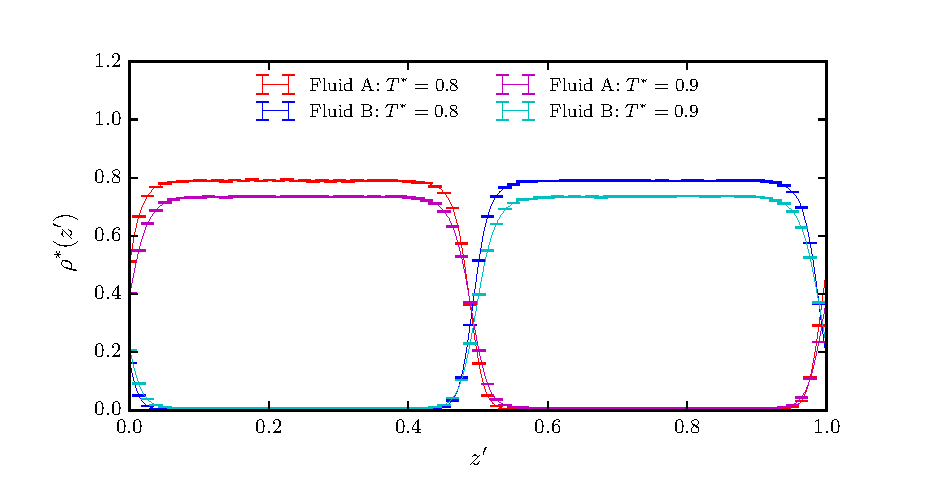
\includegraphics[scale=0.8]{Period10Rho}
\caption{Period10Rho}
\label{Period10Rho}
\end{figure}
After this period the density profile (plotted in Figure \ref{Period10Rho}) clearly showed a uniform fluid density in the fluid bulk and a sharp interfacial region as expected.
However, it is clear that the exact position of the interface had shifted slightly during the simulation and was no longer coincedent for the two temperatures.
This would have severe consequences when calculating the Marangoni force from the stress profile and thus this shift had to be manually corrected by recentering the interfaces prior to computing the finite difference
\FloatBarrier

\begin{figure}[h]
\centering
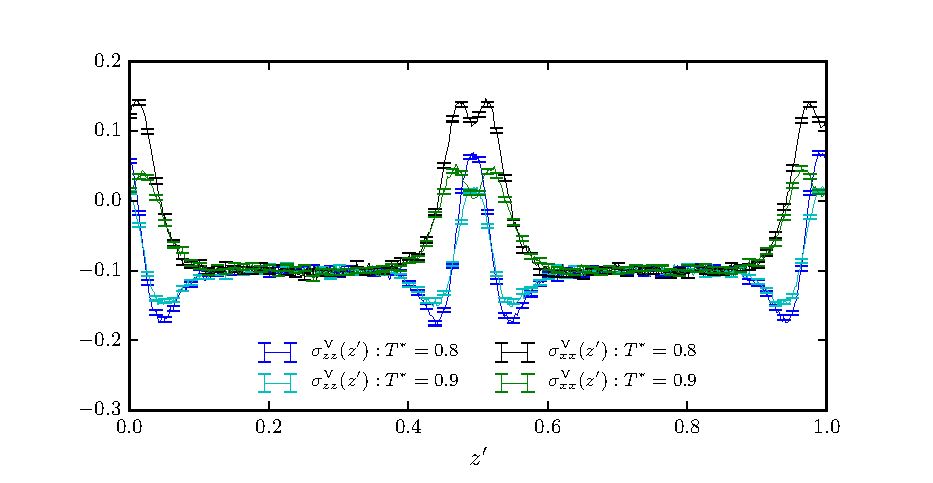
\includegraphics[scale=0.8]{Period10VirStress}
\caption{Period10VirStress}
\label{Period10VirStress}
\end{figure}

\begin{figure}[h]
\centering
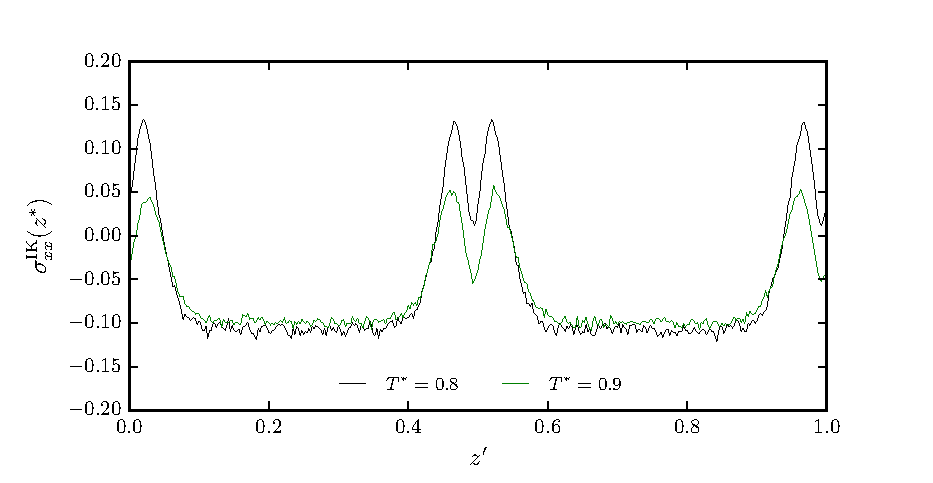
\includegraphics[scale=0.8]{Period10IKStress}
\caption{Period10IKStress}
\label{Period10IKStress}
\end{figure}
The recentered Virial and Irving--Kirkwood stress profiles are plotted in Figure \ref{Period10VirStress} and Figure \ref{Period10IKStress} respectively.
As with the fluid confined between two walls, the stress--tensor components are equal to $-P_{\mathrm{ext}}$ in the bulk of the fluid correpsonding to the hydrostatic fluid pressure.
There is a peak in both the Virial and Irving--Kirkwood stress at the interface, again as a result of the anistropy of the interparticle forces in this region.
These peaks have the same maximum value for both stress--tensors although the Irving--Kirkwood stress shows a stronger minimum directly at the interface.

\FloatBarrier
Using these force profiles the gradient of the stress with repsect to temperature was calculated from the finite difference approach.
For there to be no net force acting on the fluid there must be some source of momentum sink in the system, for example a distant wall bounding the fluid.
No such momentum sink exists for the infinite fluid represented by this system, therefore the force profile must be adjusted to give no net force.
To achieve this the average force was subtracted from the force profile fixing ensuring that the integral of the force profile over all space was zero as shown in Figure \ref{Period10Force}.

\begin{figure}[h]
\centering
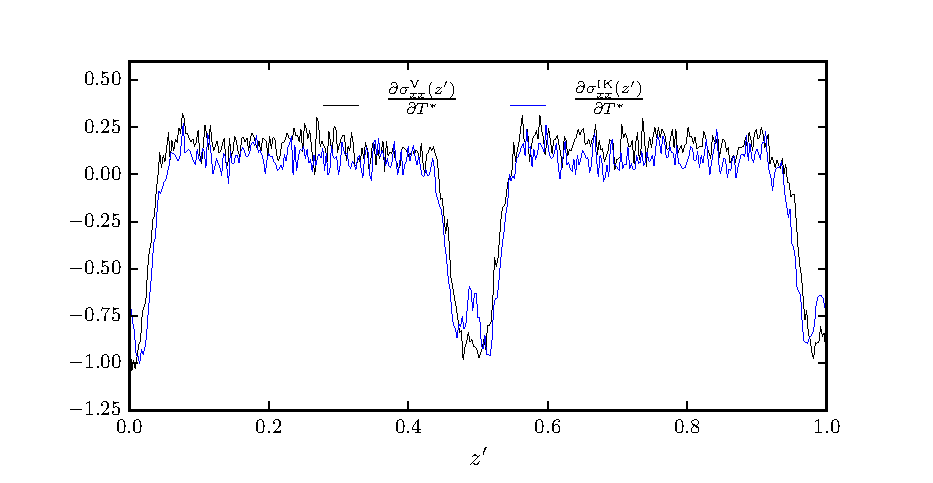
\includegraphics[scale=0.8]{Period10Force}
\caption{Period10Force}
\label{Period10Force}
\end{figure}
The resulting force profile shows a similar peak at the interface to seen in Figure \ref{PisIKForce} with a similar maximum value suggesting that fixing the total force on the fluid to zero correctly adjusts the data to give a physically meaningful Marangoni force.
Again there is a reasonably good correspondence between the force calculated using the Irving--Kirkwood and Virial stress--tensors although directly at the interface the magnitude of the peak is reduced for the Irving--Kirkwood force.
Away from the interface there is a bulk force acting in the opposite direction to the interfacial Marangoni force that will generate the expected bulk backflow.
However the profile as a whole shows too much noise for the fine--structure of the force to be determined and thus is not of a sufficient quality to be used as an artificial body--force in a non--equilibrium simulation.

\subsection{Reducing the noise in the force--profile}

 



\subsection{Using a periodic binary-mixture}
The purest system to study is the case of a symmetrical binary--mixture under three-dimensional periodic boundary conditions, whereby the only deviation from a simple bulk fluid is the presence of two interfaces within the periodic unit box. 
In this case and forces arising within the fluid can only arise from the effects of the interfaces on the fluid.

This system can be generated using a Lennard--Jones fluid by controlling the relative interaction strengths of the two fluids (henceforth referred to as Fluid A and Fluid B).
To achieve a suitable level of miscibility of the fluids the values $\epsilon_{AA} = \epsilon_{BB} = 1.0$ and $\epsilon_{AB}=0.55$ were used, in agreement with the previous studies on symmetrical Lennard--Jones binary mixtures.\cite{MorenzoRazo,Blas}
The pressure was chosen to be $P=0.1$ and the temperature values used were $T=0.8$ and $T=0.9$, ensuring that for all simulations the system exists within the liquid region of the pLennard--Jones phase space.\cite{Smit}
With an absence of any bounding walls in the system, the fluid pressure and temperature were controlled using a Nos\'{e}--Hoover barostat and thermostat.
